\documentclass[a4paper, 12pt]{article}
\usepackage{graphicx}
\usepackage{float}
\usepackage{listings}
\usepackage[UTF8]{ctex}
\usepackage{xcolor}
\setlength{\parindent}{2em}
\lstdefinestyle{mybash}{
    language=bash,                 % 设置语言为 Bash[reference:8]
    basicstyle=\small\ttfamily,    % 基础字体：使用等宽字体（即我们设置的 Consolas）[reference:9][reference:10]
    keywordstyle=\color{blue},     % 关键字颜色[reference:11][reference:12]
    keywordstyle={[2]\color{cyan}},% 第二组关键字颜色[reference:13]
    commentstyle=\itshape\color{orange!70!black}, % 注释样式：斜体 + 橙色[reference:14]
    stringstyle=\color{teal},      % 字符串颜色[reference:15]
    backgroundcolor=\color{yellow!10}, % 背景色：浅黄色[reference:16][reference:17]
    frame=single,                  % 代码框样式[reference:18]
    numbers=left,                  % 在左侧显示行号[reference:19]
    numberstyle=\tiny\color{gray}, % 行号样式[reference:20]
    breaklines=true,               % 自动换行
    showstringspaces=false,        % 不显示字符串中的空格[reference:21][reference:22]
}
\begin{document}
  \title{Week01 实验报告}
  \author{mrw1114}
  \date{August, 27th}
  \maketitle
  \section{个人信息}
  \begin{itemize}
    \item 姓名：王俊杰
    \item 学号：25020007122
    \item Github 仓库链接：https://github.com/mrw1114/fundamentals-of-system-dev-tools
  \end{itemize}
  \section{课上实验}
    \subsection{第01题：含空格文件名的批量整理}
      \subsubsection{创建 input 目录和对应的文件}
      创建目录使用 mkdir 命令；随后利用 echo 命令新建并写入文件，其中 -e 选项启用转义字符识别，-n 选项不输出换行，同时使用单引号包裹文件名确保空格被识别成文件名的一部分；接下来利用 touch 命令新建空文件；run.log 中的日志为模拟的两条日志。接下来用 ls 命令展示目录结构，其中 -alR 选项分别代表显示隐藏文件、列出详细信息、递归地显示目录及子目录内容；之后使用 cat 命令展示各文件内容
      \noindent
      \begin{figure}[H]
        \centering
        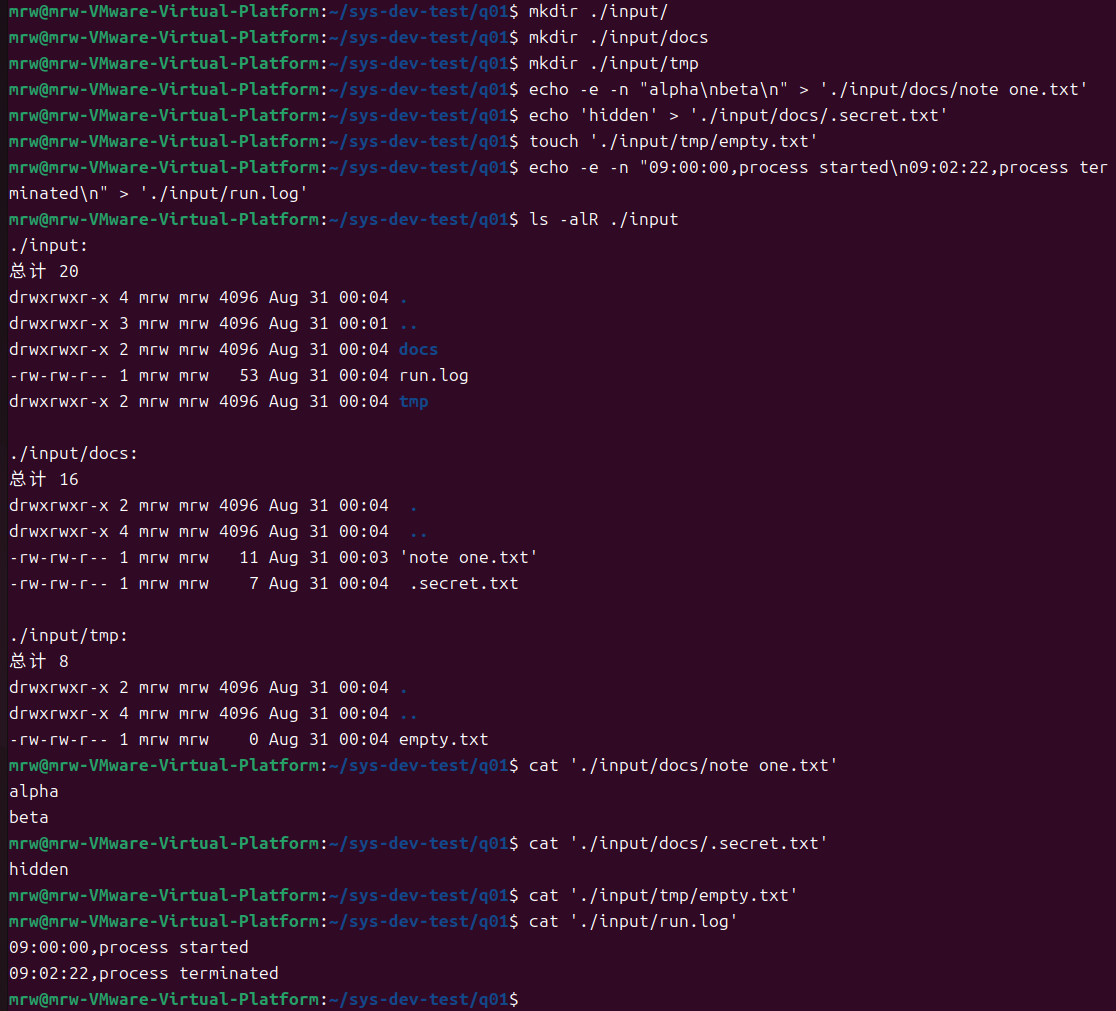
\includegraphics[width=\textwidth]{./01-1.png}
        \caption{新建操作及效果}
        \label{01-1}
      \end{figure}
      \subsubsection{显示绝对路径和 input 下全部文件}
      使用 realpath 命令来获取 q01 的真实路径，再用 ls -alR 命令列出所有文件及隐藏文件
      \noindent
      \begin{figure}[H]
        \centering
        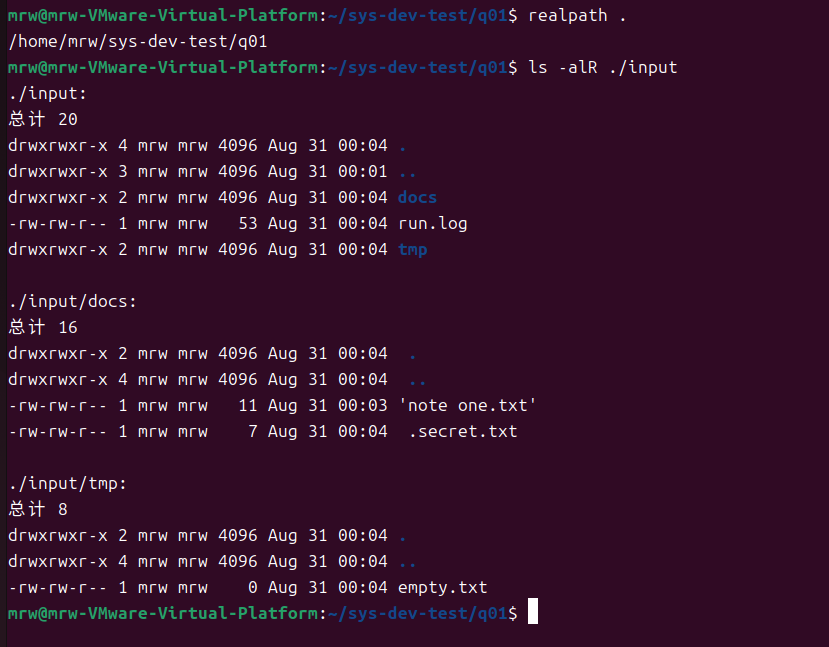
\includegraphics[width=\textwidth]{./01-2.png}
        \caption{真实路径与全部文件}
        \label{01-2}
      \end{figure}
      \subsubsection{复制 txt 文件并保留相对目录结构}
      首先新建目录 work25020007122。由于需要对目录中所有 txt 文件进行复制并保留相对结构，不能直接使用 cp 命令递归复制（会把 run.log 也一起进行复制）。可以用 find 命令和通配符查找 input 目录下的每个 txt 文件再利用 cp 命令的 \detokenize{--}parents 选项保留路径结构；其中 -type 制定查找文件的类型，f为普通文件，d为目录；-exec 表示需对被查找到的文件执行的命令，\{\} 为查找到的文件名传入的地方；\textbackslash; 表示经过转义的分号，代表命令的结束，转义是为了避免被解释为行内命令的分隔符。为确保复制的是相对路径，需要用 cd 命令进入 input 文件夹进行复制。
      \begin{figure}[H]
        \centering
        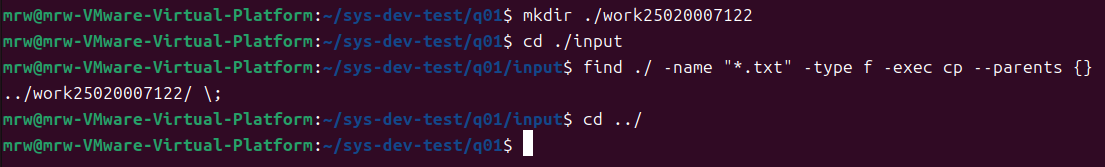
\includegraphics[width=\textwidth]{./01-3.png}
        \caption{选择性复制并保留相对结构}
        \label{01-3}
      \end{figure}
      \subsubsection{修改权限并生成总结}
      利用 find 命令查找 work25020007122 中的普通文件和目录，分别执行 chmod 750 和 chmod 640 以设置权限。再通过 find 命令的 -printf 选项生成统计总结，其中 \%p 表示含相对目录的文件名，\%s 表示文件字节数，再将得到的统计信息重定向到 inventory.txt 文件中。
      \noindent
      \begin{figure}[H]
        \centering
        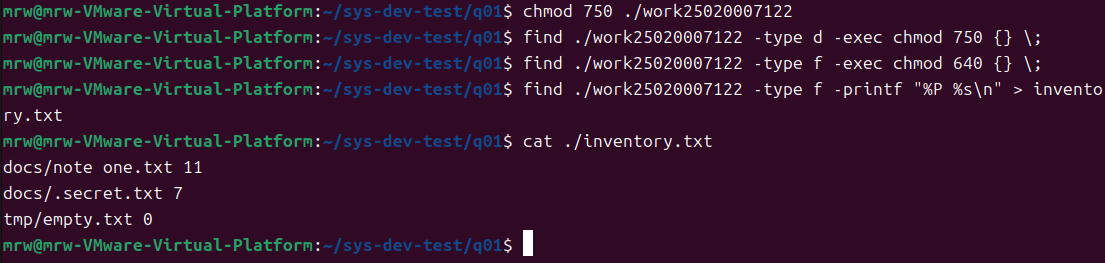
\includegraphics[width=\textwidth]{./01-4.png}
        \caption{修改权限与生成总结}
        \label{01-4}
      \end{figure}

    \subsection{第02题：随机访问日志统计}
      \subsubsection{创建 access.csv 文件}
      将测试数据写入 access.csv 文件。
      \noindent
      \begin{figure}[H]
        \centering
        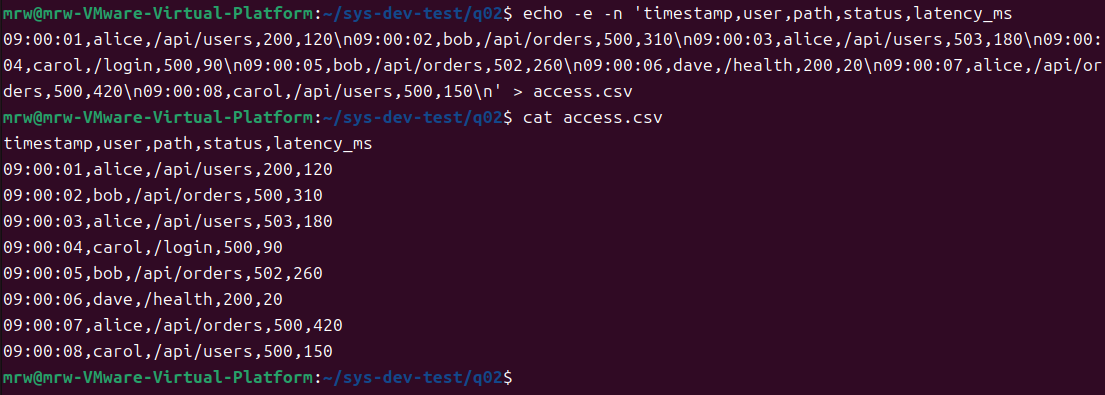
\includegraphics[width=\textwidth]{./02-1.png}
        \caption{写入 access.csv 文件}
        \label{02-1}
      \end{figure}
      \subsubsection{编写 analyse.sh 文件}
      使用 vim 工具编辑 analyse.sh 文件，随后使用 chmod 为其添加可执行权限，access.csv 文件内容如下
\begin{lstlisting}[caption={analyse.sh 的内容},style=mybash]
#!/bin/bash
# 判断是否传入1个参数
if [ $# -ne 1 ]; then
    echo "Usage: $0 <csv_file>" >&2
    exit 1
fi
# 判断是否存在文件
if [ ! -e $1 ]
then
  echo "$1 doesn't exist" >&2
  exit 2
fi

# 排序并输出5xx次数最多的 path
awk -F',' 'NR!=1&&$4>=500 {cnt[$3]++} END {for(i in cnt)print cnt[i],i}' $1 | sort -t',' -k1,1nr -k2,2 | awk -F' ' '{print $2}' | head -n 2

# 计算平均路径
awk -F',' 'NR!=1 {sum+=$5; n++} END {if(n != 0) printf "%.2f\n", sum / n; else print "0.00"}' $1
\end{lstlisting}
      其中，[ ]表示 test 命令，! 表示反转条件，-e 判断文件是否存在，-ne 表示数值是否不相等。在使用的内置变量中，\$\#表示传入的参数数量，\$1表示传入的第一个参数。此处使用 awk 指令进行数据提取与过滤，其中 -F 制定分割符， NR 表示当前行的行号，END 表示读取完每一行后才执行后面的操作，\$n （从1开始）表示第 n 列内容。sort 指令对每行内容排序，-t 指定分隔符，其中 "-k1,1nr" 表示第1个排序规则为对第1列按数据方式升序排序后反向排序（降序），k2,2表示第二个排序规则为对第二列的 path 按字典序升序排列。head -n 2 表示仅输出前两行
      \begin{figure}[H]
        \centering
        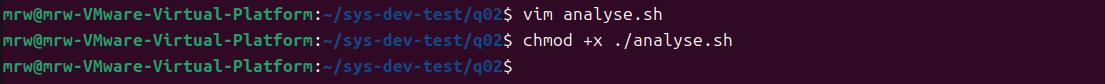
\includegraphics[width=\textwidth]{./02-2.png}
        \caption{编写 analyse.sh 并赋予其可执行权限}
        \label{02-2}
      \end{figure}
    \subsubsection{运行程序}
    分别对 access.csv 和不存在的文件 hajimi.csv 运行程序观察输出
     \begin{figure}[H]
        \centering
        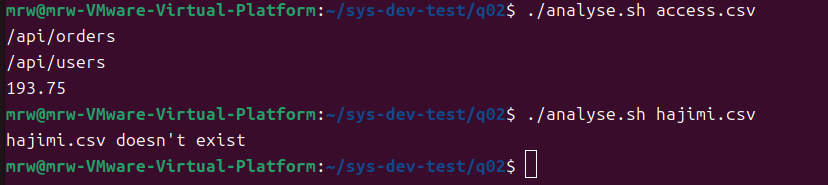
\includegraphics[width=\textwidth]{./02-3.png}
        \caption{观察运行结果}
        \label{02-3}
      \end{figure}
    \subsection{第03题：制造、解决并解释一次合并冲突}
      \subsubsection{新建仓库与初始提交}
      新建文件夹 my-repo ，进入该文件夹执行 git init 完成初始提交。安装的 git 使用 master 作为默认名称，故此处用 main 作为主分支名称。随后修改 config.txt 文件，用 git add 命令将文件加入暂存区，再使用 git commit -m 向本地仓库完成初始提交。在提交前需要使用 git config \detokenize{--}global 设置 user.name 和 user.email。
      \begin{figure}[H]
        \centering
        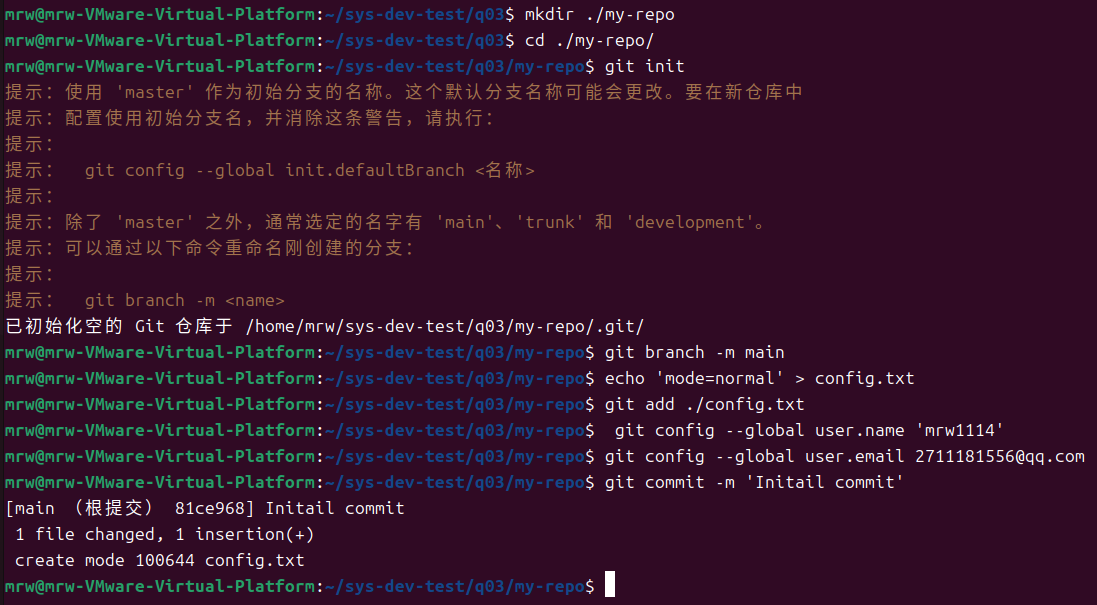
\includegraphics[width=\textwidth]{./03-1.png}
        \caption{新建仓库与初始提交}
        \label{03-1}
      \end{figure}
      \subsubsection{创建不同分支与相应提交}
      利用 git checkout -b 在 main 的基础上创建新分支 feature-a ，在该分支下改写 config.txt 为 “mode=safe” 并提交。随后用 git checkout 切换回 main ，在此基础上创建并切换到 feature-b 分支，改写 config.txt 为 “mode=fast” 并提交。
      \begin{figure}[H]
        \centering
        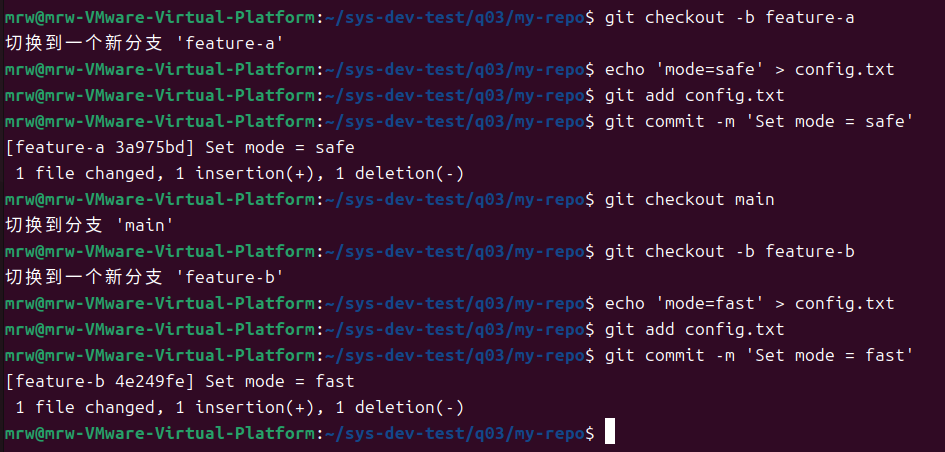
\includegraphics[width=\textwidth]{./03-2.png}
        \caption{创建两个分支并分别提交}
        \label{03-2}
      \end{figure}
      \subsubsection{冲突的制造与解决}
      回到 main 分支，用 git merge 合并 feature-a 成功，随后合并 feature-b 失败。因为两个分支都基于 main 分支且修改了同一文件的同一行。这里修改 config.txt 并 commit 来解决冲突。
      \begin{figure}[H]
        \centering
        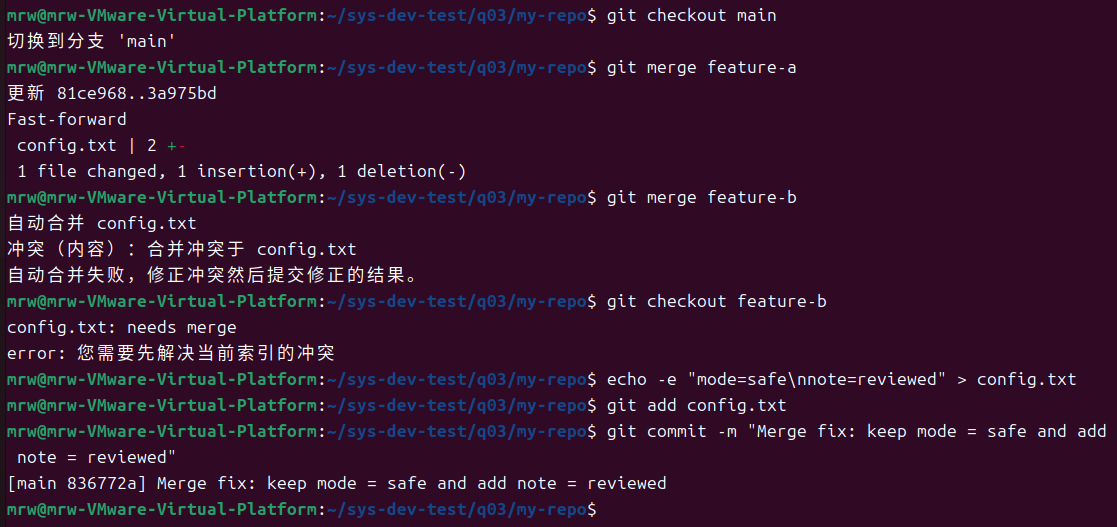
\includegraphics[width=\textwidth]{./03-3.png}
        \caption{制造与解决冲突}
        \label{03-3}
      \end{figure}
      \subsubsection{查看历史记录}
      使用 git status 查看工作区是否干净，确认干净后用制定命令查看日志。由于 feature-a 合并到 main 是 fast-forward ，所以 main 直接指向 feature-a 提交。
      \begin{figure}[H]
        \centering
        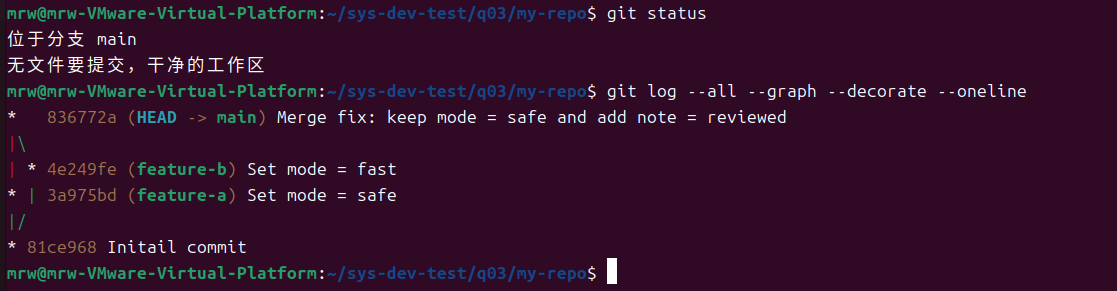
\includegraphics[width=\textwidth]{./03-4.png}
        \caption{查看状态及日志}
        \label{03-4}
      \end{figure}
    \subsection{第04题：修复并构建一页技术说明}
    \noindent
    模板中用到了中文，需要使用 ctex 宏包进行兼容。由于 pdflatex 对中文兼容性差，故采用 xelatex 进行处理。
      \subsubsection{新建模板文件}
      用 vim 将内容输入到 report.tex 中
      \begin{figure}[H]
        \centering
        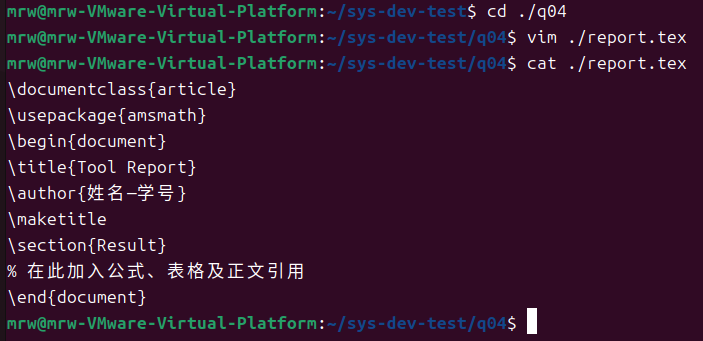
\includegraphics[width=\textwidth]{./04-1.png}
        \caption{新建 report.tex 文件}
        \label{04-1}
      \end{figure}
      \subsubsection{添加公式、表格以及引用,完善中文支持}
      添加带有编号的行间等式使用 equation，在内部使用 label 指明标签。添加表格可以先用 table 浮动块，在浮动块内使用 caption 制定标题，其后紧跟 label 指明标签，再使用 tabulor 插入表格。为了处理模板中原有的中文，需要使用 ctex 宏包。
      \begin{figure}[H]
        \centering
        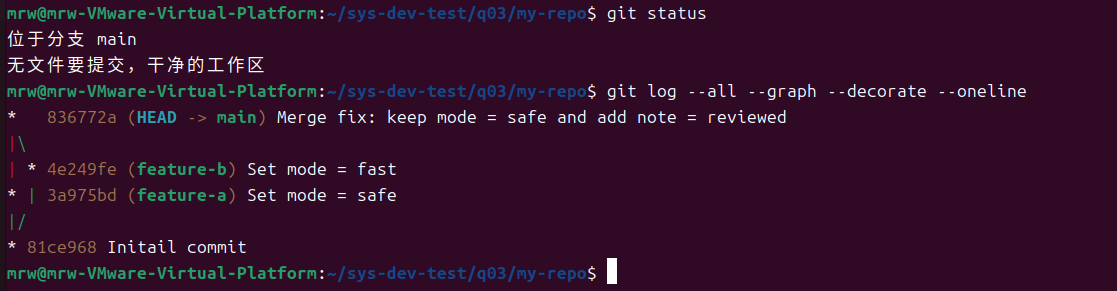
\includegraphics[width=\textwidth]{./03-4.png}
        \caption{完善 report.tex 文件}
        \label{04-2}
      \end{figure}
      \subsubsection{用 latexmk 编译输出pdf}
      由于中文兼容问题，此处使用 latexmk -xelatex -halt-on-error ./report.tex 编译 pdf。latexmk 会自动进行多次编译以保证交叉引用得以正常显示。
      \begin{figure}[H]
        \centering
        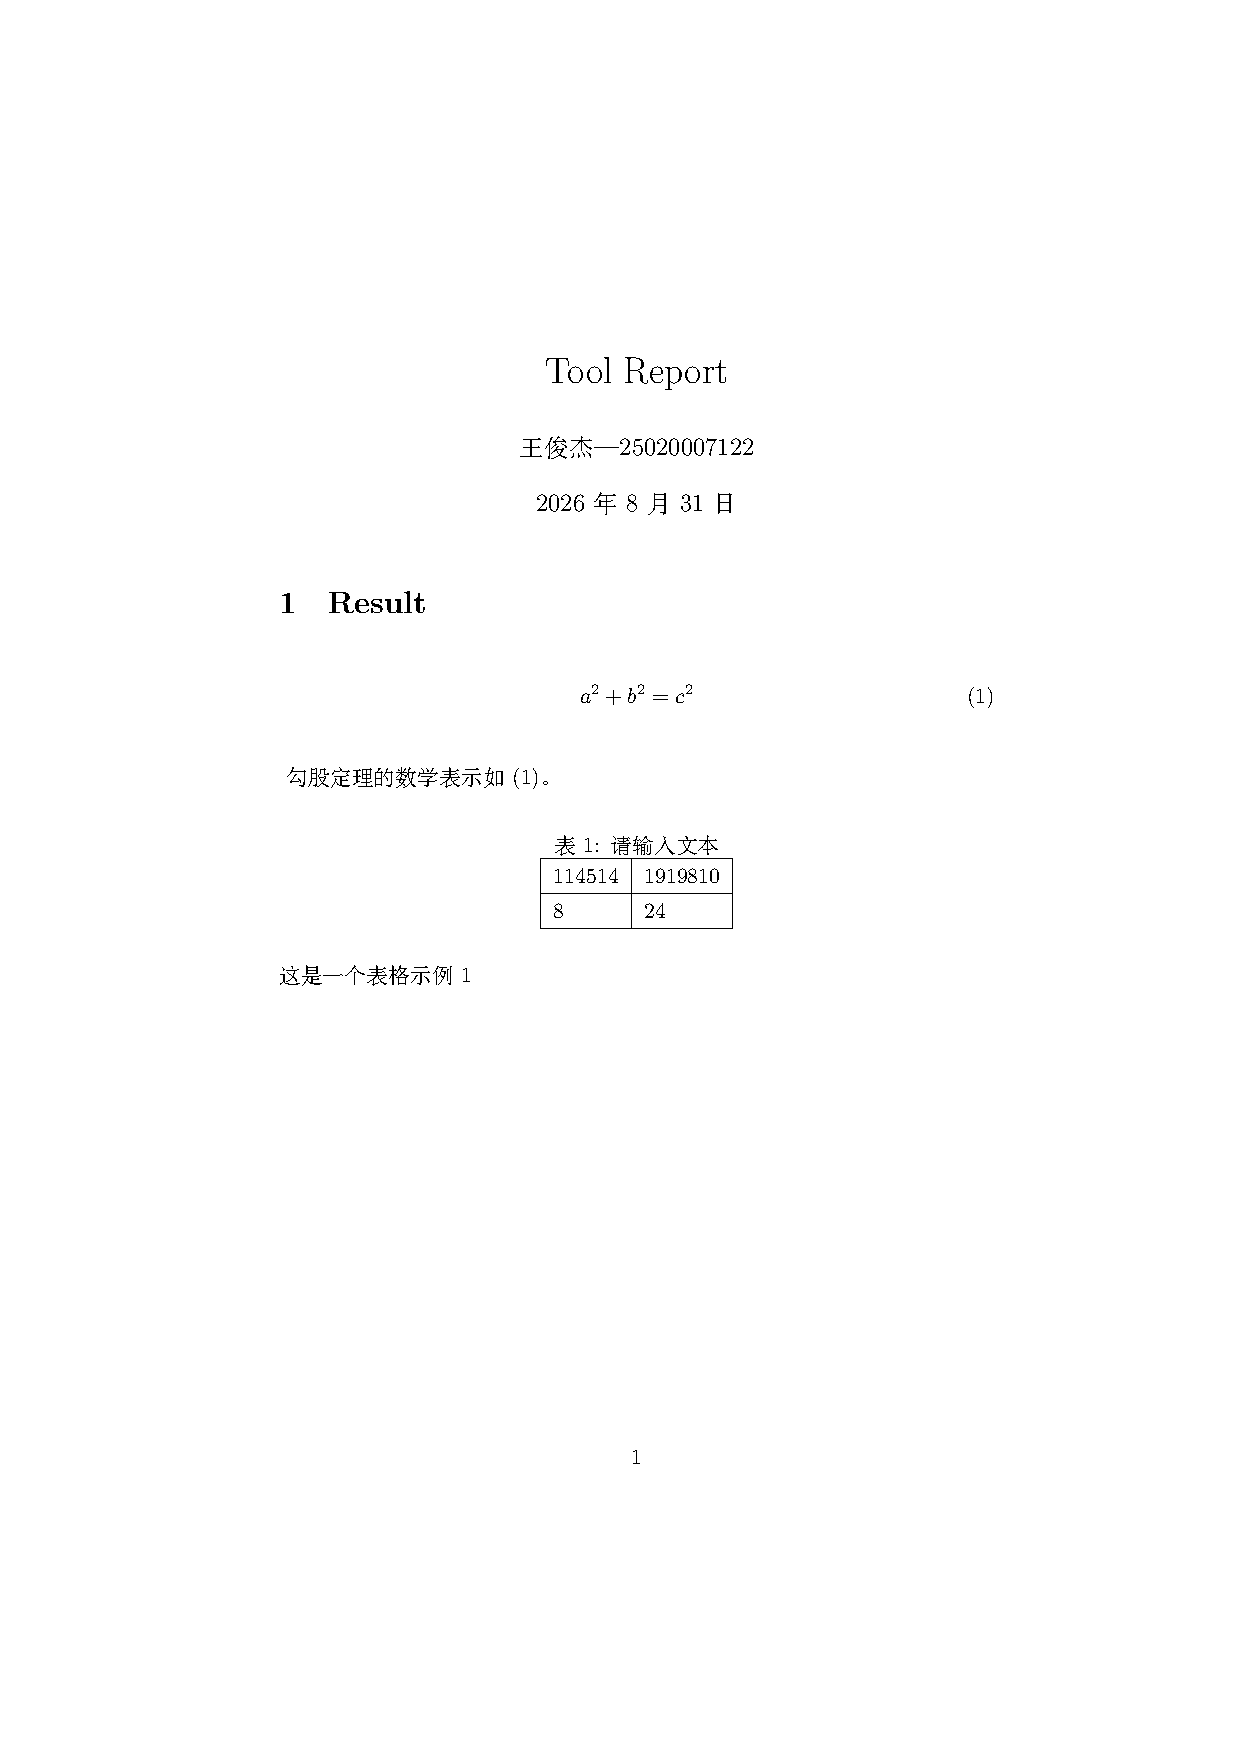
\includegraphics[width=\textwidth]{./report.pdf}
        \caption{得到的 report.pdf}
        \label{04-3}
      \end{figure}
  \section{课后练习}
    \subsection{第1题}
      \subsubsection{题目描述}
      ls 的 -l 选项（flag）作用是什么？运行 ls -l / 并观察输出。每一行最前面的 10 个字符分别代表什么？
      \subsubsection{解题过程}
      ls 的 -l 选项会输出详细信息，最前面的10个字符中，第1个字符表示文件类型（ - 为普通文件，d 为目录, l 为符号链接， b 为块设备， c 为字符设备，p 为管道，s 为套接字）之后的9个字符每3个一组，分别表示文件所有者，同用户组，其他用户的读(r)、写(w)、执行(x)权限，- 表示无该权限。其中 /tmp 目录具备 t 权限，表示所有人都能在此处创建文件但只能删除自己创建的文件。
        \begin{figure}[H]
          \centering
          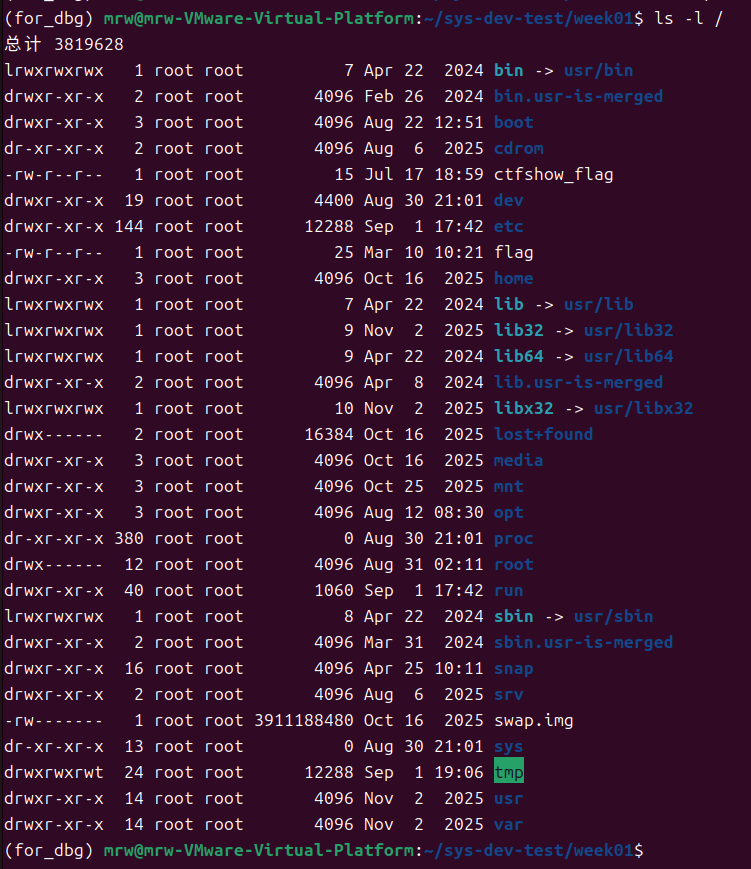
\includegraphics[width=\textwidth]{./work-01.png}
          \caption{ls -l / 输出结果}
          \label{work-01}
        \end{figure}
    \subsection{第2题} 
      \subsubsection{题目描述}
      '单引号'、"双引号" 和 \$'ANSI 引号' 有什么区别？写一条命令，输出一个同时包含字面量 \$ 、! 和换行符的字符串。
      \subsubsection{解题过程}
      单引号保留字符串内除去其自身的字符的字面量；双引号字符串会自动替换\$var为其对应的值，进行命令替换和算术替换（替换\$((expression))为expression计算所得的值）；ANSI 字符串只会对 \textbackslash 开头的转义序列进行替换。可以执行 echo \$'\$\textbackslash n!' 利用 ANSI 字符串完成任务。
        \begin{figure}[H]
          \centering
          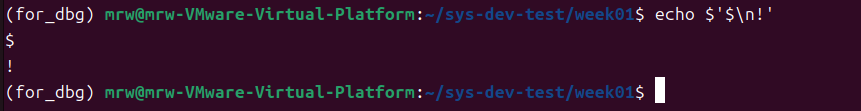
\includegraphics[width=\textwidth]{./work-02.png}
          \caption{命令输出结果}
          \label{work-02}
        \end{figure}  
    \subsection{第3题} 
      \subsubsection{题目描述}
      Shell 有三条标准流：stdin（0）、stdout（1）、stderr（2）。运行 ls /nonexistent /tmp ，把 stdout 和 stderr 分别重定向到两个文件。你将如何把两者都重定向到同一个文件？
      \subsubsection{解题过程}
      > 默认对输出流重定向到下一个参数对应的文件，x>\&y 表示将 x 指向的文件重定向到 y 指向的文件，则可以通过 ls /nonexistent /tmp > stdout.log 2> stderr.log 完成第一个任务，通过 ls /nonexistent /tmp > all.log 2>\&1 完成第二个任务（先重定向 stdout 再重定向 stderr 到 stdout 指向的文件）。
        \begin{figure}[H]
          \centering
          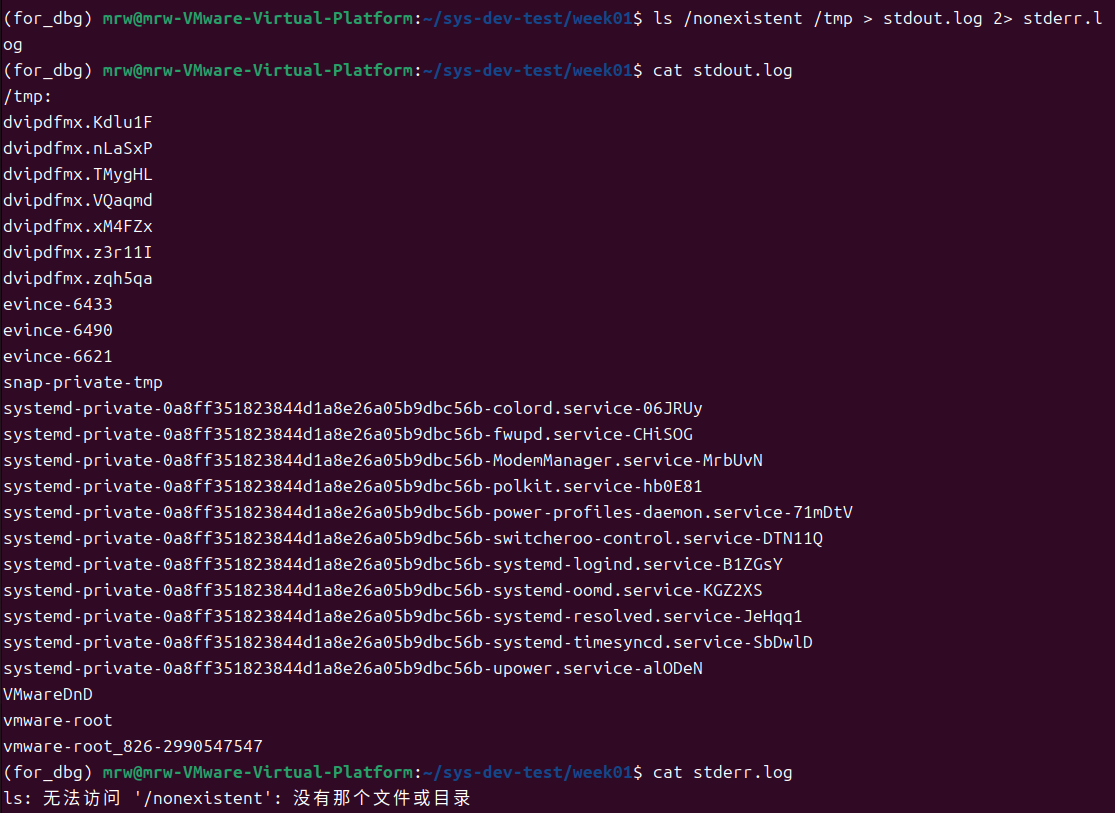
\includegraphics[width=\textwidth]{./work-03-1.png}
          \caption{第一条命令的效果}
          \label{work-03-1}
        \end{figure}
        \begin{figure}[H]
          \centering
          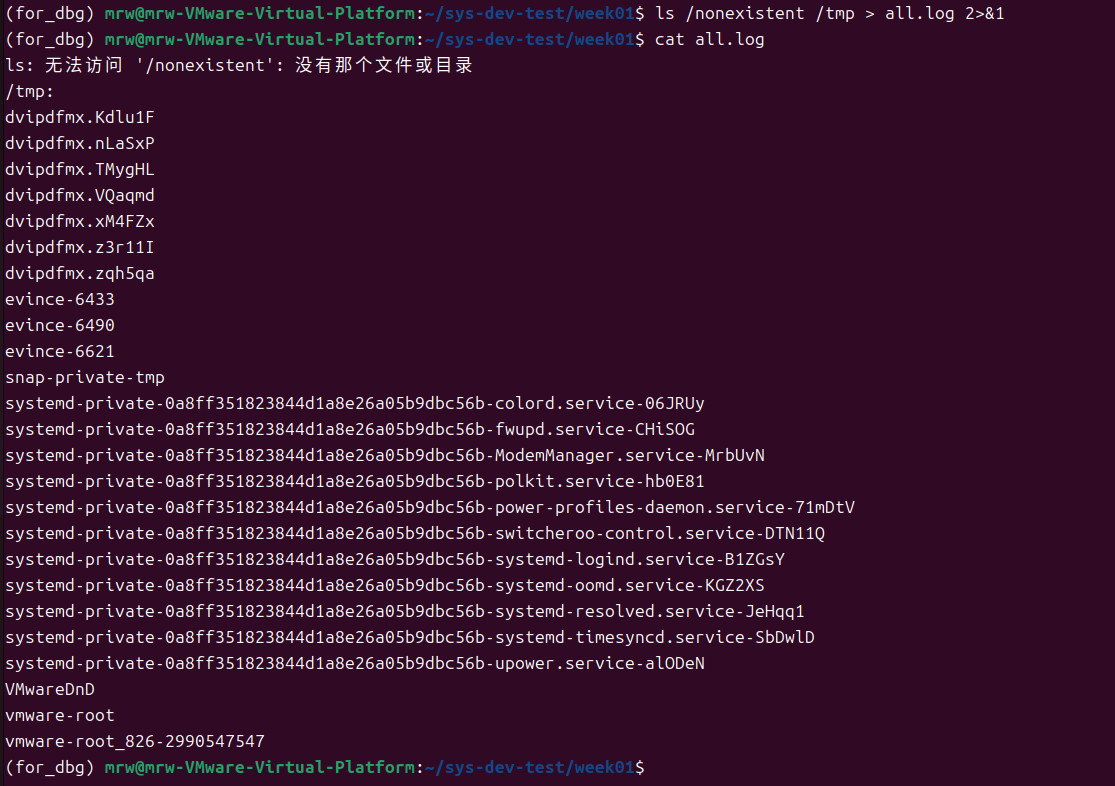
\includegraphics[width=\textwidth]{./work-03-2.png}
          \caption{第二条命令的效果} 
          \label{work-03-2}
        \end{figure}
    \subsection{第4题} 
      \subsubsection{题目描述}
      \$? 保存上一条命令的退出状态（0 表示成功）。\&\& 仅在前一条成功时执行后一条；|| 仅在前一条失败时执行后一条。写一个一行命令：仅当 /tmp/mydir 不存在时才创建它。
      \subsubsection{解题过程}
      可以利用 test 命令，其选项 -d 可以判断下一个参数对应的文件是否为目录，可以使用 [ -d /tmp/mydir ] || mkdir /tmp/mydir 来实现任务。
        \begin{figure}[H]
          \centering 
          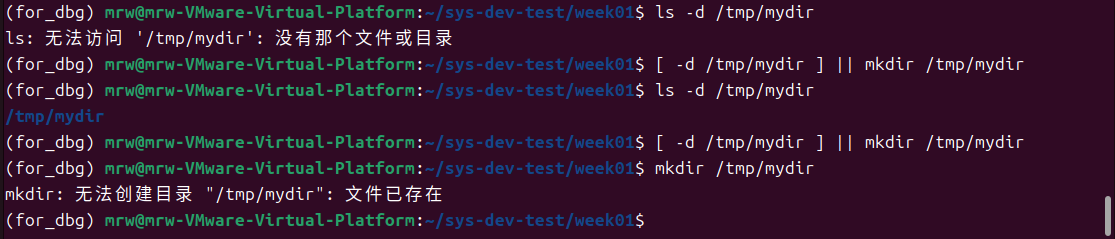
\includegraphics[width=\textwidth]{./work-04.png}
          \caption{命令执行效果}
          \label{work-04}
        \end{figure}
    \subsection{第5题} 
      \subsubsection{题目描述}
      为什么 cd 必须是 Shell 内建命令，而不能是独立程序？
      \subsubsection{解题过程}
      shell 在执行独立可执行程序时会创建子进程来执行，而子进程仅能修改和父进程共同占有的内核资源（指向同一个文件描述符所对应的偏移，管道等），无法修改父进程的内存空间、环境变量、工作目录、默认权限掩码、进程资源限制。若将 cd 设置为独立程序，被执行时只能修改自己子进程的工作目录，而无法修改作为父进程的 shell 的工作目录。所以 cd 仅能作为 shell 的内建命令。
    \subsection{第6题} 
      \subsubsection{题目描述}
      在脚本的 set 选项（flag）里加入 -x 会发生什么？写个简单脚本试试并观察输出。
      \subsubsection{解题过程}
      set -x 会打开调试模式，执行命令时会先显示提示符 '+' （加号的数量代表是在第几层子 shell 里执行，仅有一个就是当前 shell ）和被执行的命令和参数（经过变量替换等）再执行命令。
        \begin{figure}[H]
          \centering 
          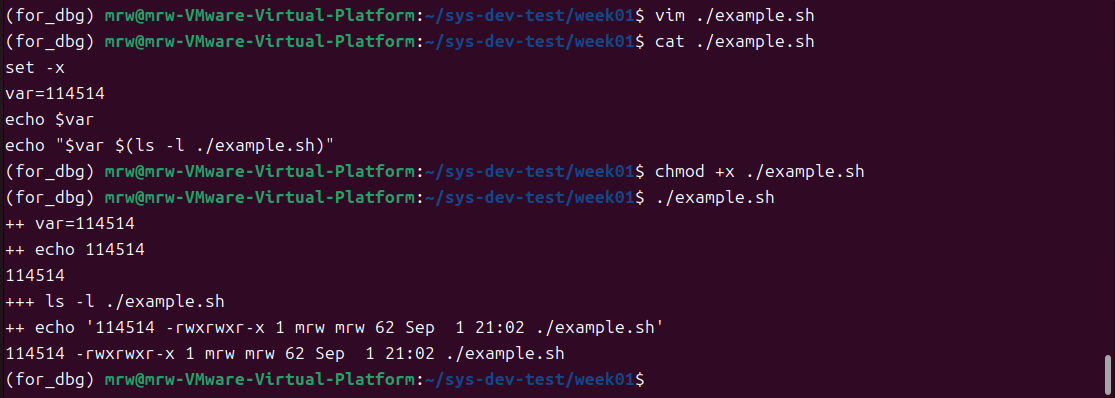
\includegraphics[width=\textwidth]{./work-06.png}
          \caption{脚本执行效果}
          \label{work-06}
        \end{figure}
    \subsection{第7题} 
      \subsubsection{题目描述}
      写一条命令，把文件复制为带当天日期的备份文件名（例如 notes.txt → notes\_2026-01-12.txt）
      \subsubsection{解题过程}
      date 命令可以输出当天日期，则使用命令替换可以实现目的，如 cp notes.txt "notes\_\$(date +\%Y-\%m-\%d).txt"。
        \begin{figure}[H]
          \centering
          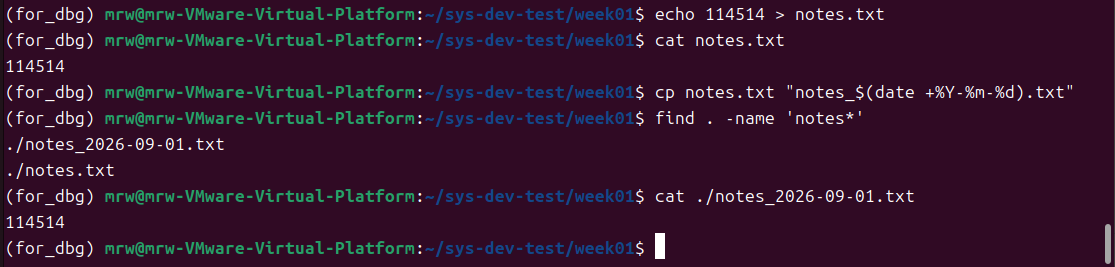
\includegraphics[width=\textwidth]{./work-07.png}
          \caption{文件备份效果}
          \label{work-07}
        \end{figure}
    \subsection{第8题} 
      \subsubsection{题目描述}
      使用管道找出你「home 目录」中最常见的 5 种文件扩展名。（提示：组合 find 、grep / sed / awk、sort、uniq -c 以及 head）
      \subsubsection{解题过程}
      利用 find 命令查找家目录下的含后缀名的文件，利用 sed 和正则表达式匹配并删除最后一个点前的内容，利用 sort 对得到的后缀名排序，使用 uniq -c 统计每行对应的次数，用 sort 命令对次数降序排序，最后用 head 命令输出前5行。可以使用 find ~ -type f -name "*.*" | sed 's/.*\textbackslash.//' | sort | uniq -c | sort -nr | head -5 来完成任务。
        \begin{figure}[H]
          \centering
          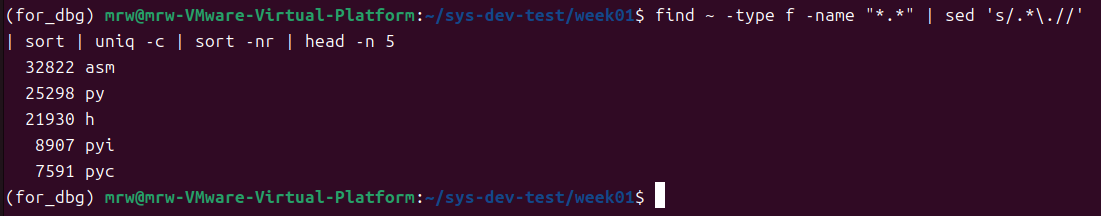
\includegraphics[width=\textwidth]{./work-08.png}
          \caption{后缀名统计结果}
          \label{work-08}
        \end{figure}
    \subsection{第9题} 
      \subsubsection{题目描述}
      xargs 会把 stdin 的每一行转换为命令参数。结合 find 和 xargs（不要用 find -exec），找出目录中所有 .sh 文件，并用 wc -l 统计每个文件行数。加分项：正确处理文件名中的空格。（提示：-print0 和 -0）参见 man xargs 。
      \subsubsection{解题过程}
      利用 find 和通配符 *.sh 可以发现后缀为 .sh 的文件，但是 find 默认用换行分隔结果而 xargs 默认以空格分隔参数。故 -print0 让 find 以 \textbackslash0 分隔结果，-0 让 xargs 按 \textbackslash 划分参数。可以使用 find . -name '*.sh' -print0 | xargs -0 wc -l 来完成任务。
        \begin{figure}[H]
          \centering
          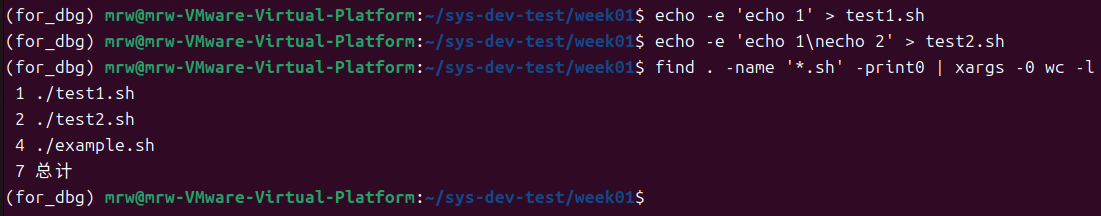
\includegraphics[width=\textwidth]{./work-09.png}
          \caption{.sh 文件统计结果}
          \label{work-09}
        \end{figure}
    \subsection{第10题} 
      \subsubsection{题目描述}
      awk 可以按列值过滤行并改写输出。例如，awk '\$3 \~ /pattern/ \{\$4=""; print\}' 会只输出第三列匹配 pattern 的行，并省略第四列。请写一个 awk 命令：只输出第二列大于 100 的行，并交换第一列和第三列。可用这条命令测试：printf 'a 50 x\textbackslash nb 150 y\textbackslash nc 200 z\textbackslash n'
      \subsubsection{解题过程}
      awk 默认按空格分隔列，通过 \$n 表示第 n 行。使用 printf 'a 50 x\textbackslash nb 150 y\textbackslash nc 200 z\textbackslash n' | awk '\$2 > 100 \{print \$3, \$2, \$1\}' 来完成任务。
        \begin{figure}[H]
          \centering
          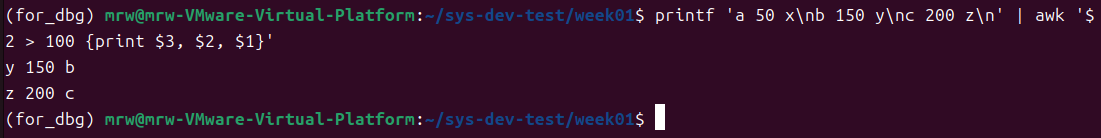
\includegraphics[width=\textwidth]{./work-10.png}
          \caption{awk 统计结果}
          \label{work-10}
        \end{figure}
    \subsection{第11题} 
      \subsubsection{题目描述}
      写一个脚本，接收文件名参数（\$1），用 test -f 或 [ -f ... ] 检查该文件是否存在，并根据结果输出不同提示。
      \subsubsection{解题过程}
      脚本如下所示
\begin{lstlisting}[caption={IsExistent.sh 的内容},style=mybash]
#!/bin/bash
# 判断是否传入1个参数
if [ $# -ne 1 ]; then
    echo "Usage: $0 <csv_file>" >&2
    exit 1
fi
# 不存在文件时
if [ ! -e $1 ]
then
  echo "$1 doesn't exist" >&2
  exit 2
fi
# 存在文件时
echo "$1 exists."
\end{lstlisting}
        \begin{figure}[H]
          \centering
          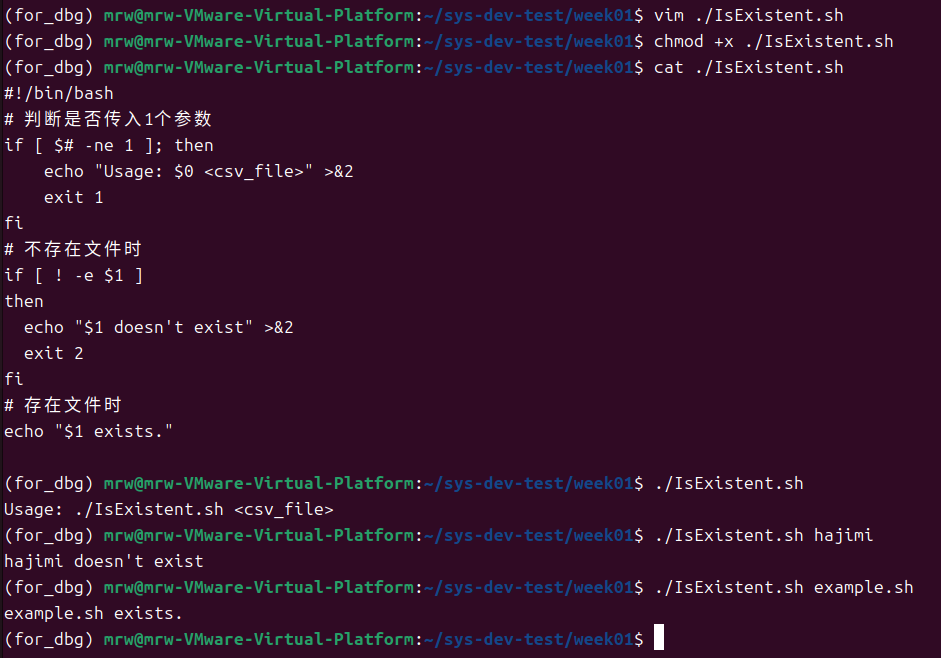
\includegraphics[width=\textwidth]{./work-11.png}
          \caption{脚本运行结果}
          \label{work-11}
        \end{figure}
  \section{commit 记录}
  \noindent
  Commit 历史截图如图所示，具体 Commit 内容可访问仓库查看。
  \begin{figure}[H]
    \centering
    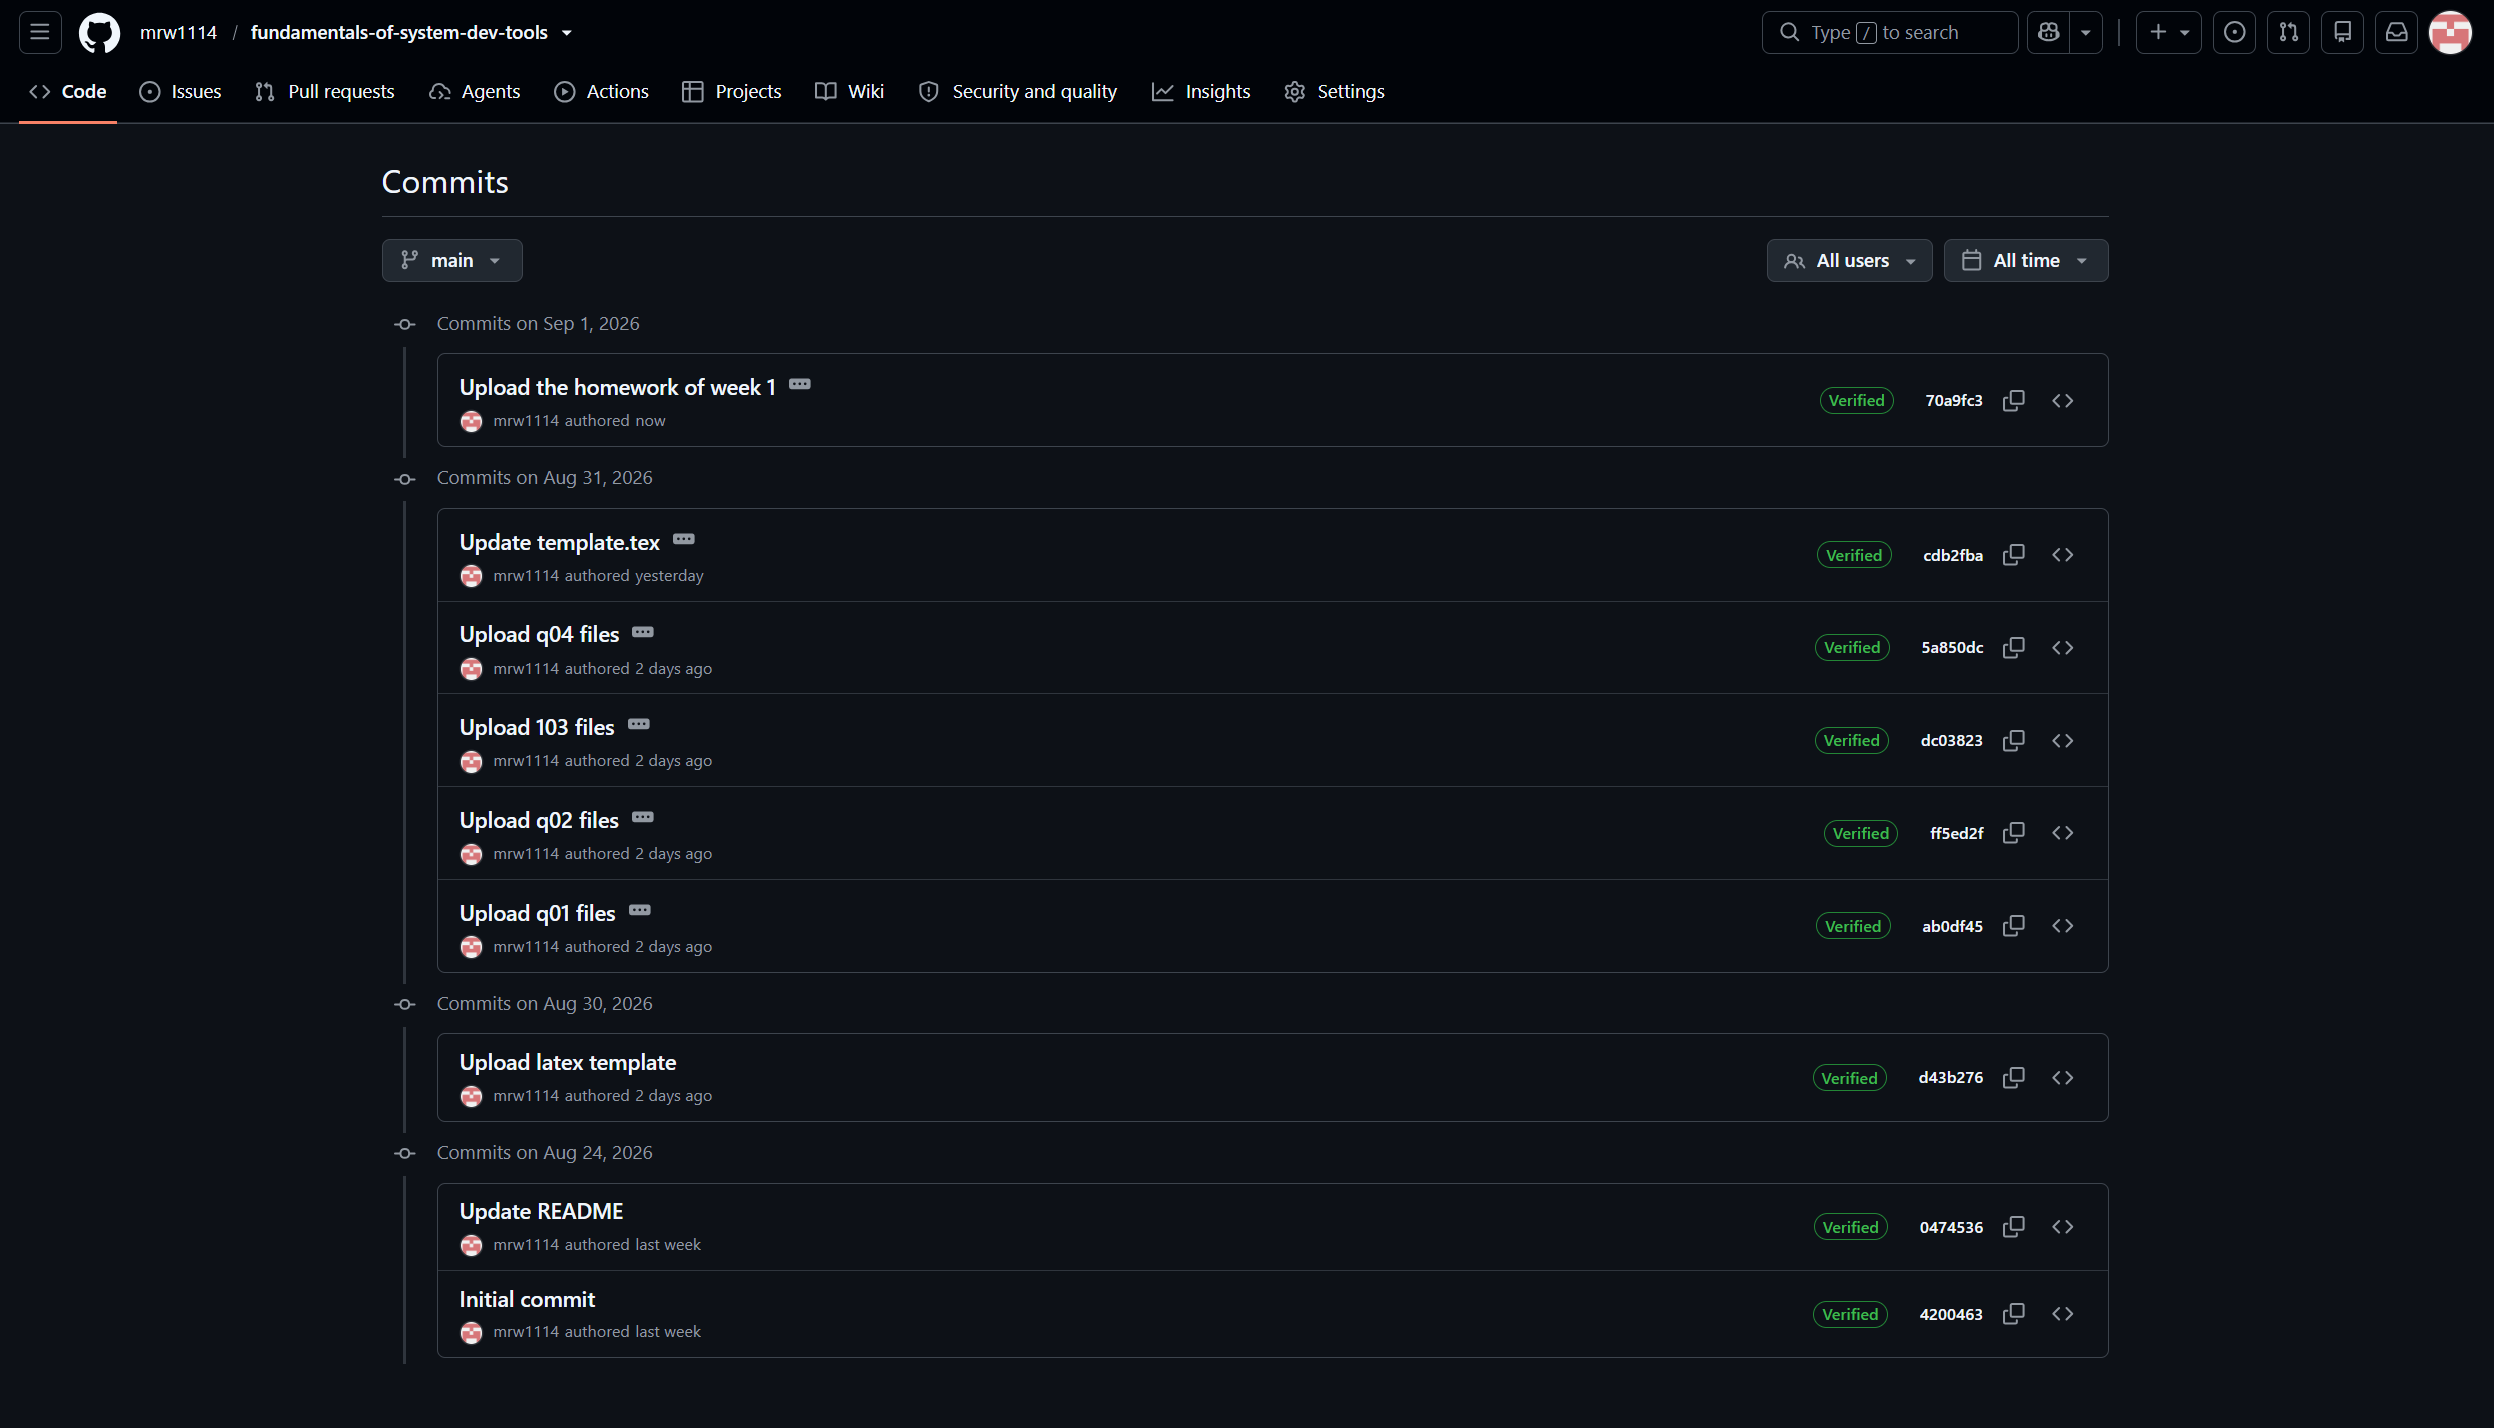
\includegraphics[width=\textwidth]{./history1.png}
    \caption{Commit 历史记录}
    \label{history1}
  \end{figure}
\end{document}
